% latexmk -pvc -pdf
\documentclass[9pt, a4paper]{article}
\usepackage[margin=0.65in]{geometry}
\usepackage{graphicx}
\usepackage{caption}
\usepackage{amsmath,amsthm,amsfonts,amssymb}
\usepackage{blindtext}
\usepackage[english]{babel}
\newenvironment{Figure}
    {\par\medskip\noindent\minipage{\linewidth}}
    {\endminipage\par\medskip}

\title{Simulating phase contrast imaging for materials with variable density}
\author{Ana C. Fabela Hinojosa \\
\small{Supervisors: Assoc. Prof. Marcus Kitchen}}
\small{\date{\today,  \\Due date: Friday 23\textsuperscript{th} September, 2021}}

\begin{document}
\maketitle
\section{Current objective}

In this project, I study the theoretical perspective of coherent X-ray imaging. Using simulations, I aim to determine whether a density difference alone can give phase contrast and, if so, whether it is likely to be detected in real experiments. I created several simulations of cylinder-shaped sample materials and subjected these samples to X-ray wave-fields of different energies. In some of my simulations, I use a single cylinder made of a homogeneous material. In others I use two embedded concentric cylinder-shaped samples of materials with either an equal chemical composition and different densities or, different chemical compositions, and densities. 
With these simulations I demonstrate the importance of material density in phase contrast imaging and by 1) showing how distinctly, phase contrast arises between material boundaries designed to mimic the grey and white matter of the brain and 2) whether the observed phase contrast is density-dependent. The eventual aim is to verify if successful phase retrieval is possible for such samples given variable sample material densities.

\section{Theory fundamentals}
For the single cylinder simulations I use the projection approximation to solve a partial differential equation known as the transport-of-intensity equation (TIE). This equation describes the relationship between the intensity and phase distribution in an optical system, and hence it can be used to quantify the contrast (i.e. refractive (phase) effects) present in propagation-based X-ray phase contrast images\cite{PagsTutes}.
\begin{equation}\label{eq:1}
-\nabla_{T} [I(x, y, z) \nabla_{T} \phi(x, y, z)] = k \frac{\partial I (x, y, z)}{\partial z},
\end{equation}
where $k$ is the wave-number, $I(x, y, z)$ is the intensity and $\phi(x, y, z)$ is the phase of the X-ray beam.
The projection approximation takes into account, X-ray--matter interaction, therefore the position dependent and complex form of the refractive index is introduced: $n(x, y, z) = 1 - \delta(x, y, z) + i \beta(x, y, z)$. The real part of this complex quantity corresponds to the refractive index, while the imaginary part is related only to the absorptive properties of the sample\cite{PagsTutes}.
Under the projection approximation, the Beer-Lambert law of attenuation is used to describe the attenuation of intensity within the sample,
\begin{equation}\label{eq:2}
I(x, y, z_0) = \mathrm{exp}[-\int_{t} \mu(x, y, z) dz] I(x, y, 0),
\end{equation}
where $\mu = 2k\beta$ is the \textit{linear attenuation coefficient} of the sample and constitutes the imaginary part of the sample's complex refractive index.
The real part of the complex refractive index ($\delta$) is known as the refractive index decrement, describing phase-shifts in the wave-front which continuously accumulate in the direction of propagation
\begin{equation}\label{eq:3}
\Delta \phi(x, y) = -k \int_{t}\delta(x, y, z)dz,
\end{equation}
where $t$ is the projected thickness of the object in the direction of the light flow.
The TIE effects observable changes onto the intensity (eq.\ref{eq:2}) and phase (eq.\ref{eq:3}) after these are used as the initial conditions of the propagation problem.

To implement the spatial evolution in the direction of the wave-front propagation, I use the fourth-order Runge-Kutta with the TIE. I employ the Runge-Kutta evolution algorithm as
\begin{equation} \label{eq:4}
\begin{split}
&k_1 = f(z, I_n, \phi),\\
&k_2 = f(z + \frac{\Delta z}{2}, I_n + \frac{1}{2}k_1, \phi)),\\
&k_3 = f(z + \frac{\Delta z}{2}, I_n + \frac{1}{2}k_2, \phi)),\\
&k_4 = f(z + \Delta z, I_n + k_3, \phi)),\\
&I_{n + 1} = I_{n} + \frac{1}{6}(k_1 + 2k_2 + 2k_3 + k_4) + O(\Delta z^5),\\
\end{split}
\end{equation}
where the spatial evolution step is set as $\Delta z = 1$~mm. The propagation via fourth order Runge-Kutta over a spatial interval is done by solving a differential equation $f$ using four Euler-style steps (i.e. the $k_i$ coefficients) where each Euler-style step involves one evaluation of the differential equation with slightly different input parameters. This method combines the information obtained for each solution to match a Taylor series expansion up to fourth order. The combined evaluations of the differential equation eliminate the error terms order by order, resulting in the remaining error being very small\cite{N_R}.

For the two-cylinder simulations, I also use the projection approximation, but this time I model the propagation of the monochromatic X-ray wave-field using a method known as the angular spectrum formulation (ASF). This method uses Fourier decomposition of wave-fields at a single plane into distinct component plane waves. Each plane wave component is propagated through the Fourier domain to a destination plane, and then the propagated wave-field components are reconstructed via an inverse spatial Fourier transform\cite{Goodman}. To implement the ASF, I use the X-ray imaging XRI library, since the existing algorithm has already implemented several fixes to undesirable instabilities that can appear in the simulations. This library was built by the Monash X-ray imaging group.

\subsection{Imaging brain structures}
The optical properties of grey and white matter are extremely similar. However, it is known that there is a small difference in the values of the attenuation coefficients of these materials. CT brain imaging has been reported to yield clearly demarcated tissue borders at the grey/white matter boundaries\cite{Beltran2}. I want to determine if density differences alone would create phase contrast or whether phase contrast is dependent on both density and material differences.
To simulate grey and white matter, I use the attenuation coefficients for both materials $\mu_{GM},\mu_{WM}$ obtained from CT imaging of rabbit and kitten brain samples. This data was acquired at Japan's SPring-8 synchrotron radiation facility using an X-ray energy of $E = 24$keV and a sample-to-detector distance of $5$m\cite{Linda}. In my calculations, I also use experimental grey and white matter densities reported in the ``IT’IS Database for thermal and electromagnetic parameters of biological tissues" (see reference \cite{ITIS}). To find the complex refractive index components of the whole brain (i.e. $\delta_B$ and $\mu_B$) under certain energy X-rays, I use the X-ray imaging group ``X-ray attenuation calculator" which employs the values recorded in NIST in database 66\cite{NIST} making these easily accessible via a GUI, (note: I use this specific tool in all my simulations, not only the ones pertaining the brain materials). 
Using all these tools I calculated an approximate estimate for the grey and white matter refractive index decrements ($\delta_{GM}$ and $\delta_{WM}$) The calculations were simple. In one, I modelled the refractive index decrements as proportional to the ratio of the attenuation coefficient value for the full brain from reference\cite{NIST} and the density of the grey or white matter values reported in reference \cite{ITIS} (for example for grey matter: $\delta_{GM} = \frac{\mu_B}{\rho_{GM}} \delta_B$). In contrast, my second model considered the refractive index decrement to be solely proportional to the ratio between the attenuation coefficient value for the full brain and the value corresponding to either the grey or white matter attenuation coefficients (for example for grey matter: $\delta_{GM} = \frac{\mu_B}{\mu_{GM}} \delta_B$). 

\section{Current results}
\subsection{Simulating a single homogeneous cylinder}
I solved the TIE in two-dimensions using the projection approximation to establish my initial conditions. My method applies the fourth order Runge-Kutta evolution algorithm described earlier, to propagate the intensity of the monochromatic scalar electromagnetic wave-field over a total distance in meters. Originally, my code discretised a two-dimensional space as an array with dimensions $x, y = 1024, 512$. I first attempted to solve the TIE in Fourier space. To calculate the wave-field's derivative terms in equation (\ref{eq:1}), I used the Fourier derivative theorem to write the derivatives. I defined functions describing the geometry and, optical properties (i.e. refractive index: $\delta(x, y, z)$ and $\mu(x, y, z)$) of the simulated cylinder. Both $\delta$ and $\mu$ functions use a sigmoid function with adjustable gradient to slightly blur the edge of the cylinder and, avoid instability while solving the integrals in equations (\ref{eq:2}) and (\ref{eq:3}). My method was slow due to the Fourier derivatives, and the output intensity profile after propagation did not appear very stable, as several instability oscillations can be seen in figure \ref{fig:1}, to fix this issue, I adjusted the ratio of the spacings in my discretised space several times to make sure that the Nyquist mode of the TIE was resolved adequately. Nevertheless I was unable to obtain a completely smooth, and realistic looking intensity profile in figure \ref{fig:1}.
\begin{Figure}\label{fig:1}
\centering
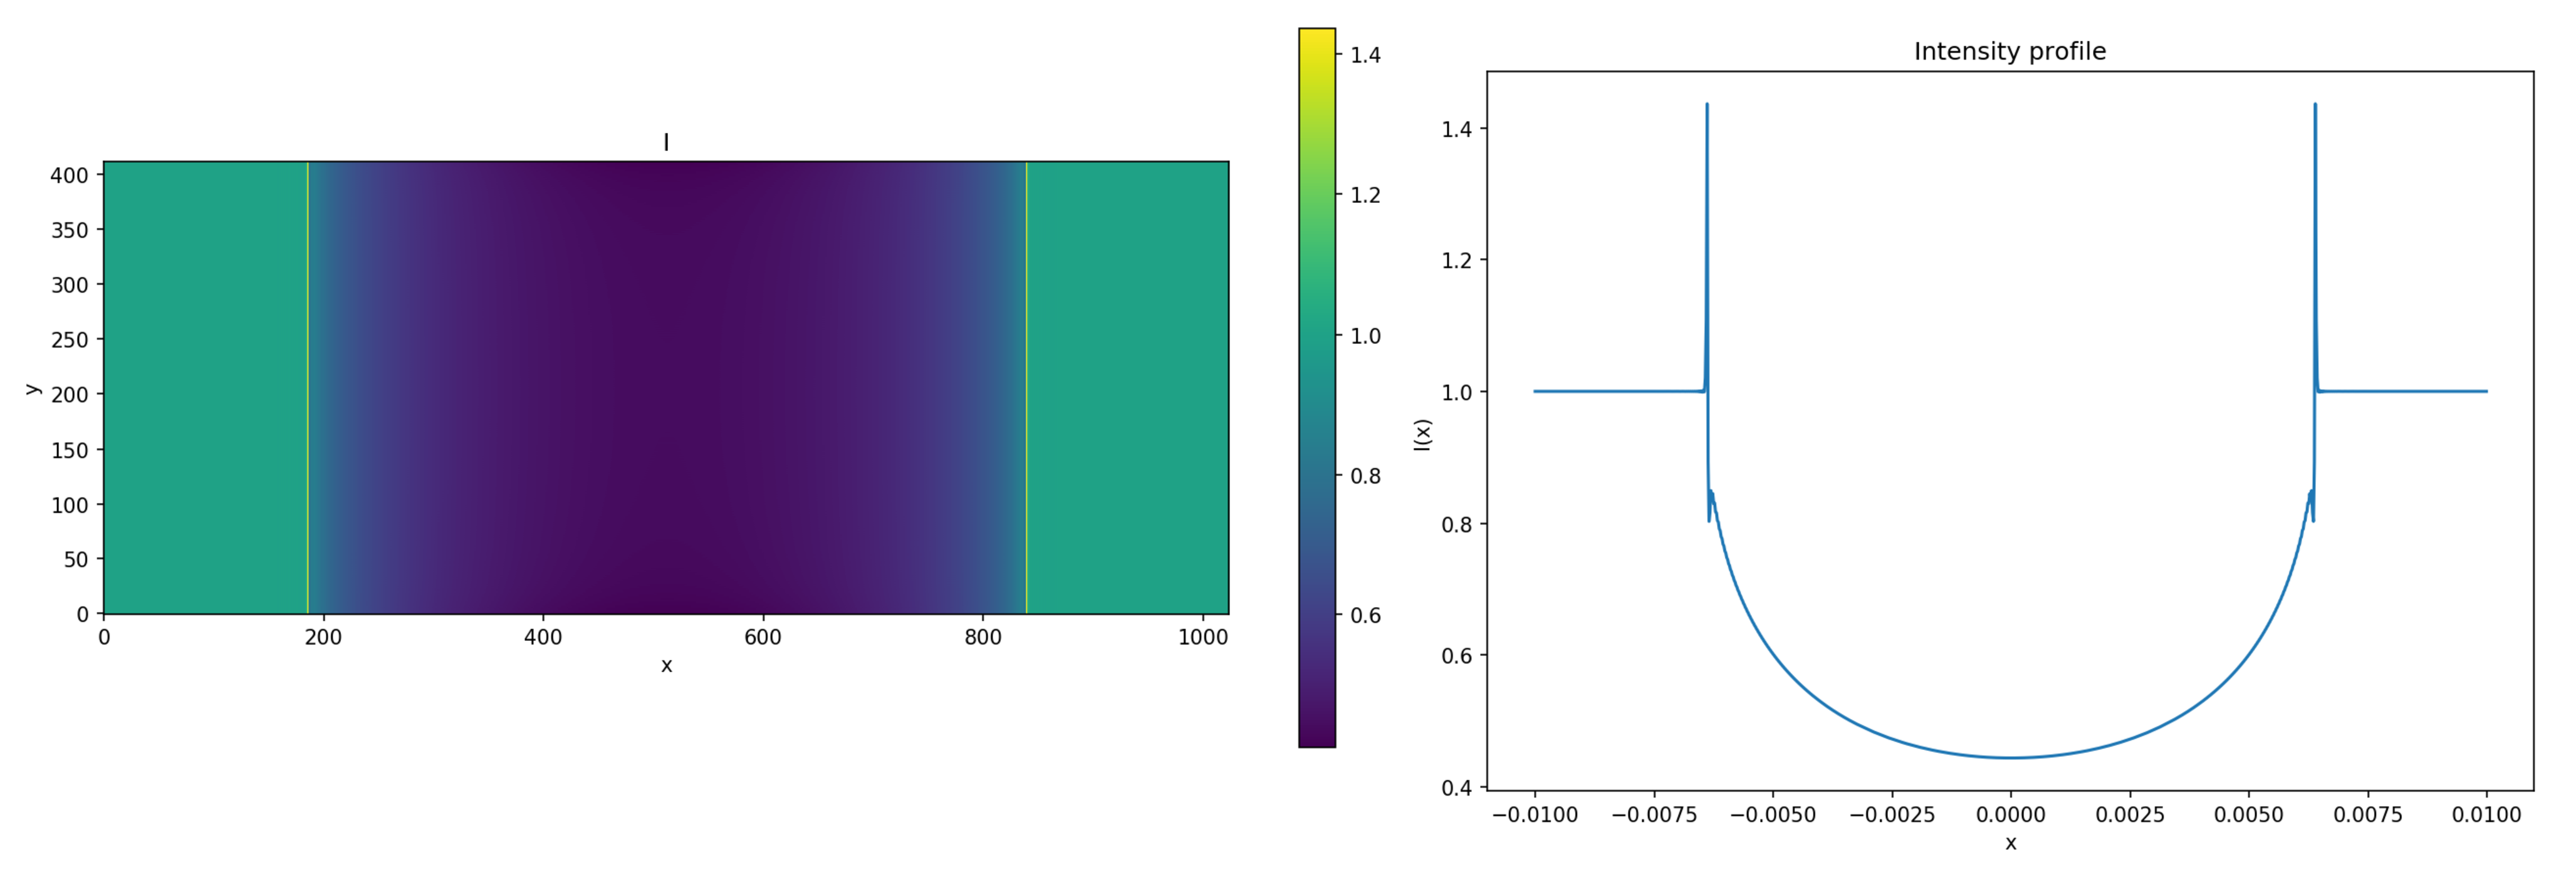
\includegraphics[width=\linewidth]{Fourier_intensity_profile.pdf}
\captionof{figure}{Phase contrast image (a), cross section (b), and enhanced view of (b) showing small ringing artefacts (instability)(c) obtained using the Fourier TIE method. This method was not able to simultaneously match the expected phase contrast peak height, given this energy and, sample material parameters while at the same time remaining fully stable. The parameters used to obtain this image were an X-ray energy of $22.1629$ keV (corresponding to a Ag k-alpha 1 source), a refractive index decrement for the water cylinder of $\delta = 4.68141\times10^{-7}$ and an attenuation coefficient of $\mu = 64.38436~\mathrm{m^{-1}}$. The cylinder radius was $R = 6.375$ mm. The sigmoid function blurred $0.5$ pixels over the edge of the imaged cylinder. The propagation distance used was $z = 1$ m.}
\end{Figure}

To complement this investigation, I took a slightly different approach and solved the TIE in position space using finite differences. I use \texttt{numpy.gradient} to evaluate each derivative and \texttt{scipy.ndimage.laplace} to evaluate the phase Laplacian term in the TIE. My code discretised the two-dimensional space as a 2D array $x, y = 1024, 1024$. 
The probable underlying reason why my Fourier method didn't work as expected was due to an effect known as Gibbs phenomenon, this effect occurs when the nth partial sum of a Fourier series undergoes large oscillations near regions with jump discontinuities\cite{Gibbs} (i.e. like the phase contrast fringes). Discovering that higher degree polynomial interpolation does not always improve accuracy was interesting and certainly unexpected.
\begin{Figure}\label{fig:2}  
\centering
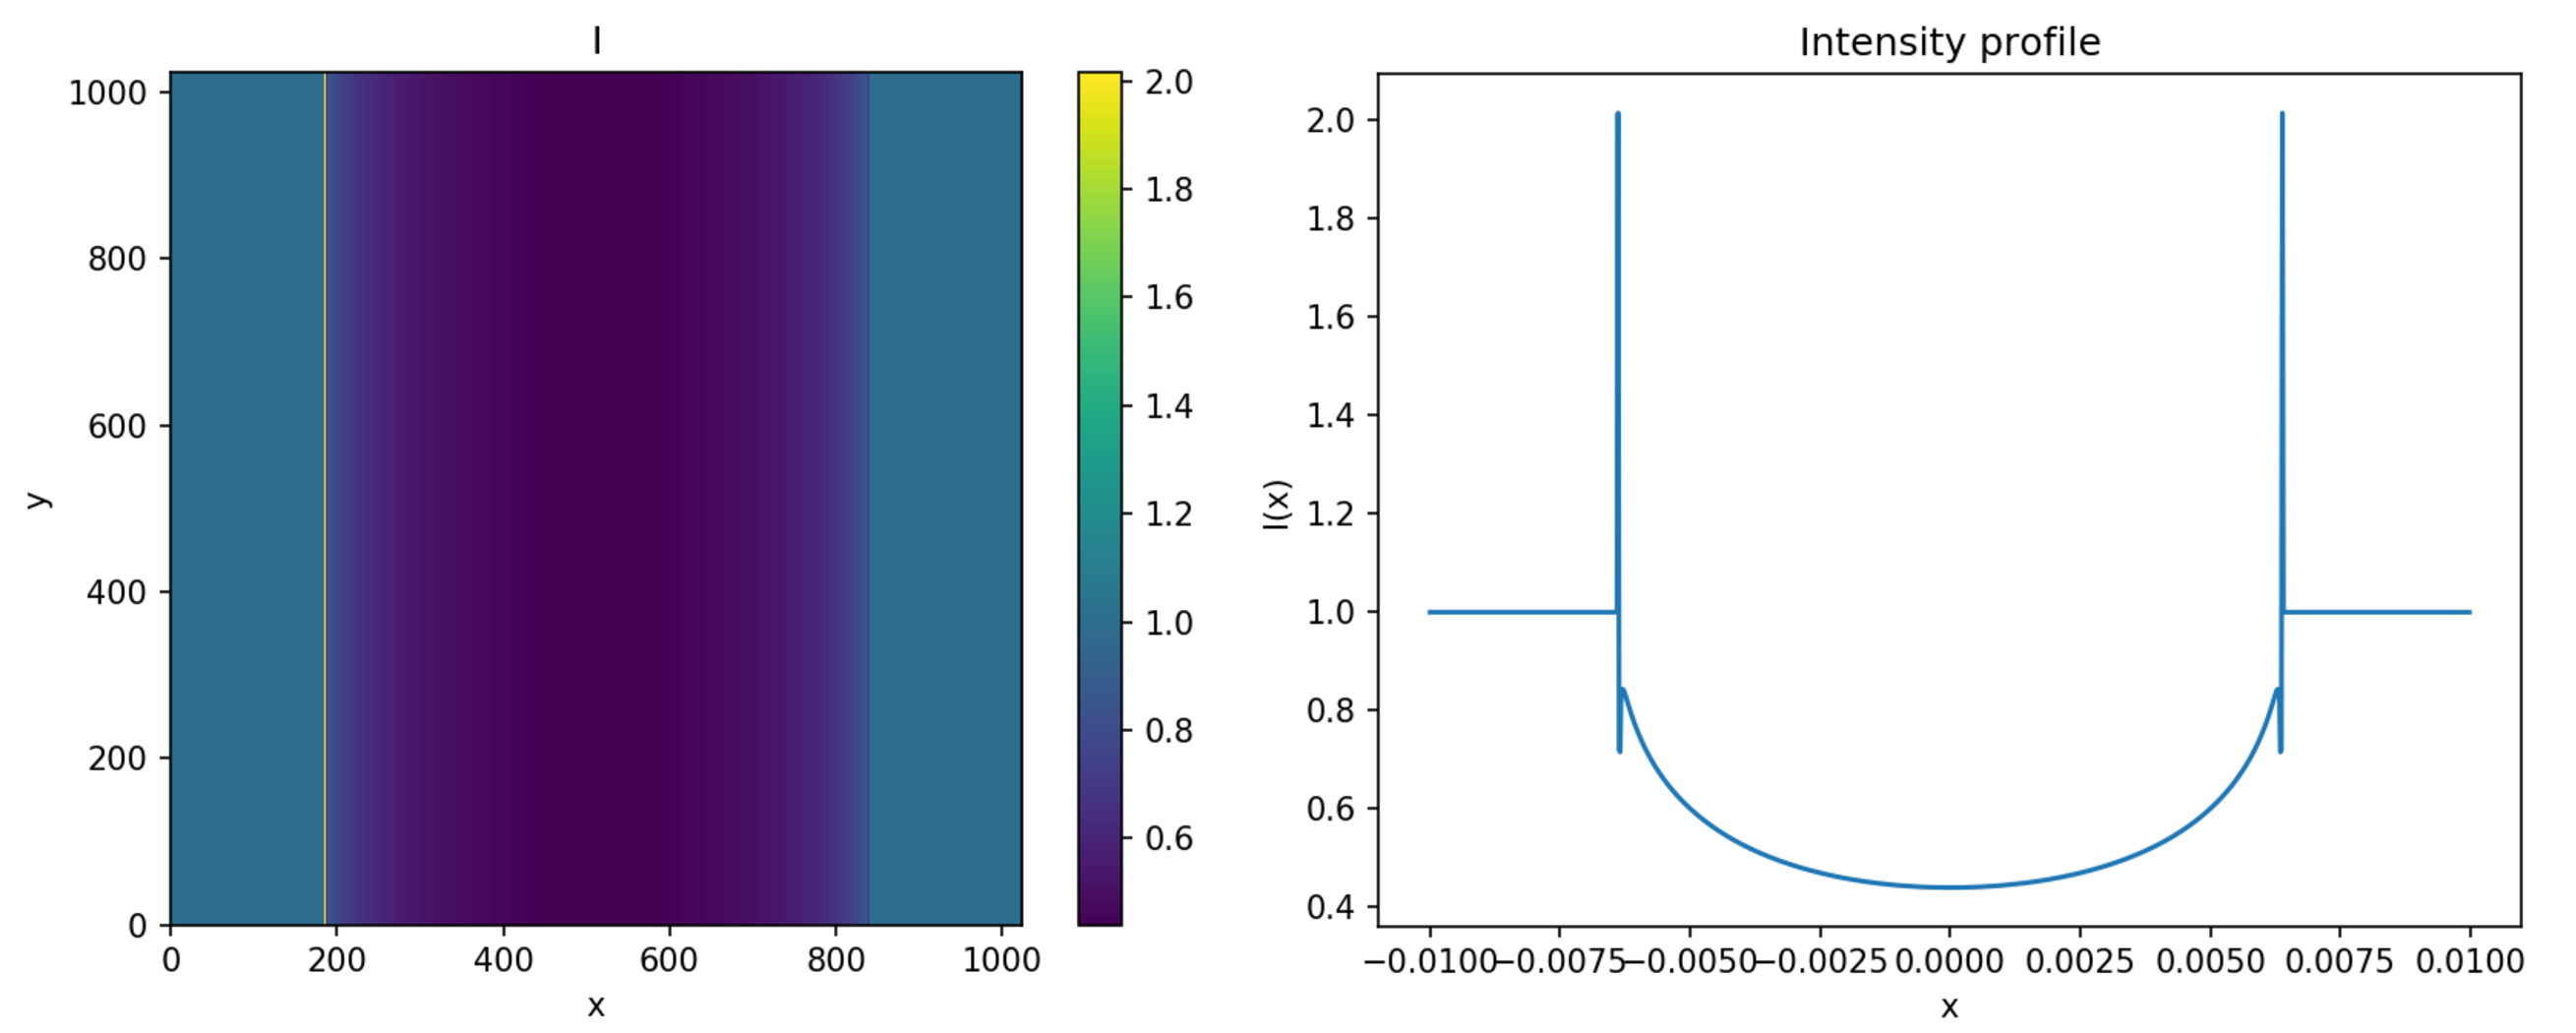
\includegraphics[width=\linewidth]{FD_intensity_profile.pdf}
\captionof{figure}{Phase contrast image and cross section obtained using finite differences and Runge-Kutta. As can be seen here, the phase contrast peaks are much higher than the profile found using the Fourier method in figure \ref{fig:1}. The parameters used to obtain this image were an X-ray energy of $22.1629$ keV (corresponding to a Ag k-alpha 1 source), a refractive index decrement for the water cylinder of $\delta = 4.68141\times 10^{-7}$ and an attenuation coefficient of  $\mu = 64.38436~\mathrm{m^{-1}}$. The cylinder radius was $R = 6.375$ mm. The sigmoid function blurred $0.14$ pixels over the edge of the imaged cylinder. The propagation distance used was $z = 1$ m. The apparent asymmetry of the two-dimensional phase contrast image is due to aliasing.}
\end{Figure}
This result presented an apparent improvement in the height of the expected phase contrast fringes. Because of this, I made sure  and made sure that all input parameters were the equal as those used in the code I used to compare my outputs (the script I used for comparisons was was made by my supervisor).

\subsection{Testing if Runge-Kutta propagation increases phase contrast}

In figure \ref{fig:3}, I obtain phase contrast cross sections from solving the TIE using my finite-difference--Runge-Kutta method and the finite difference method developed by the x-ray imaging group. I demonstrate that my method returns a smooth, and realistic looking phase contrast cross section with higher phase contrast than that returned by the X-ray group's method. 

\begin{Figure}\label{fig:3}
\centering
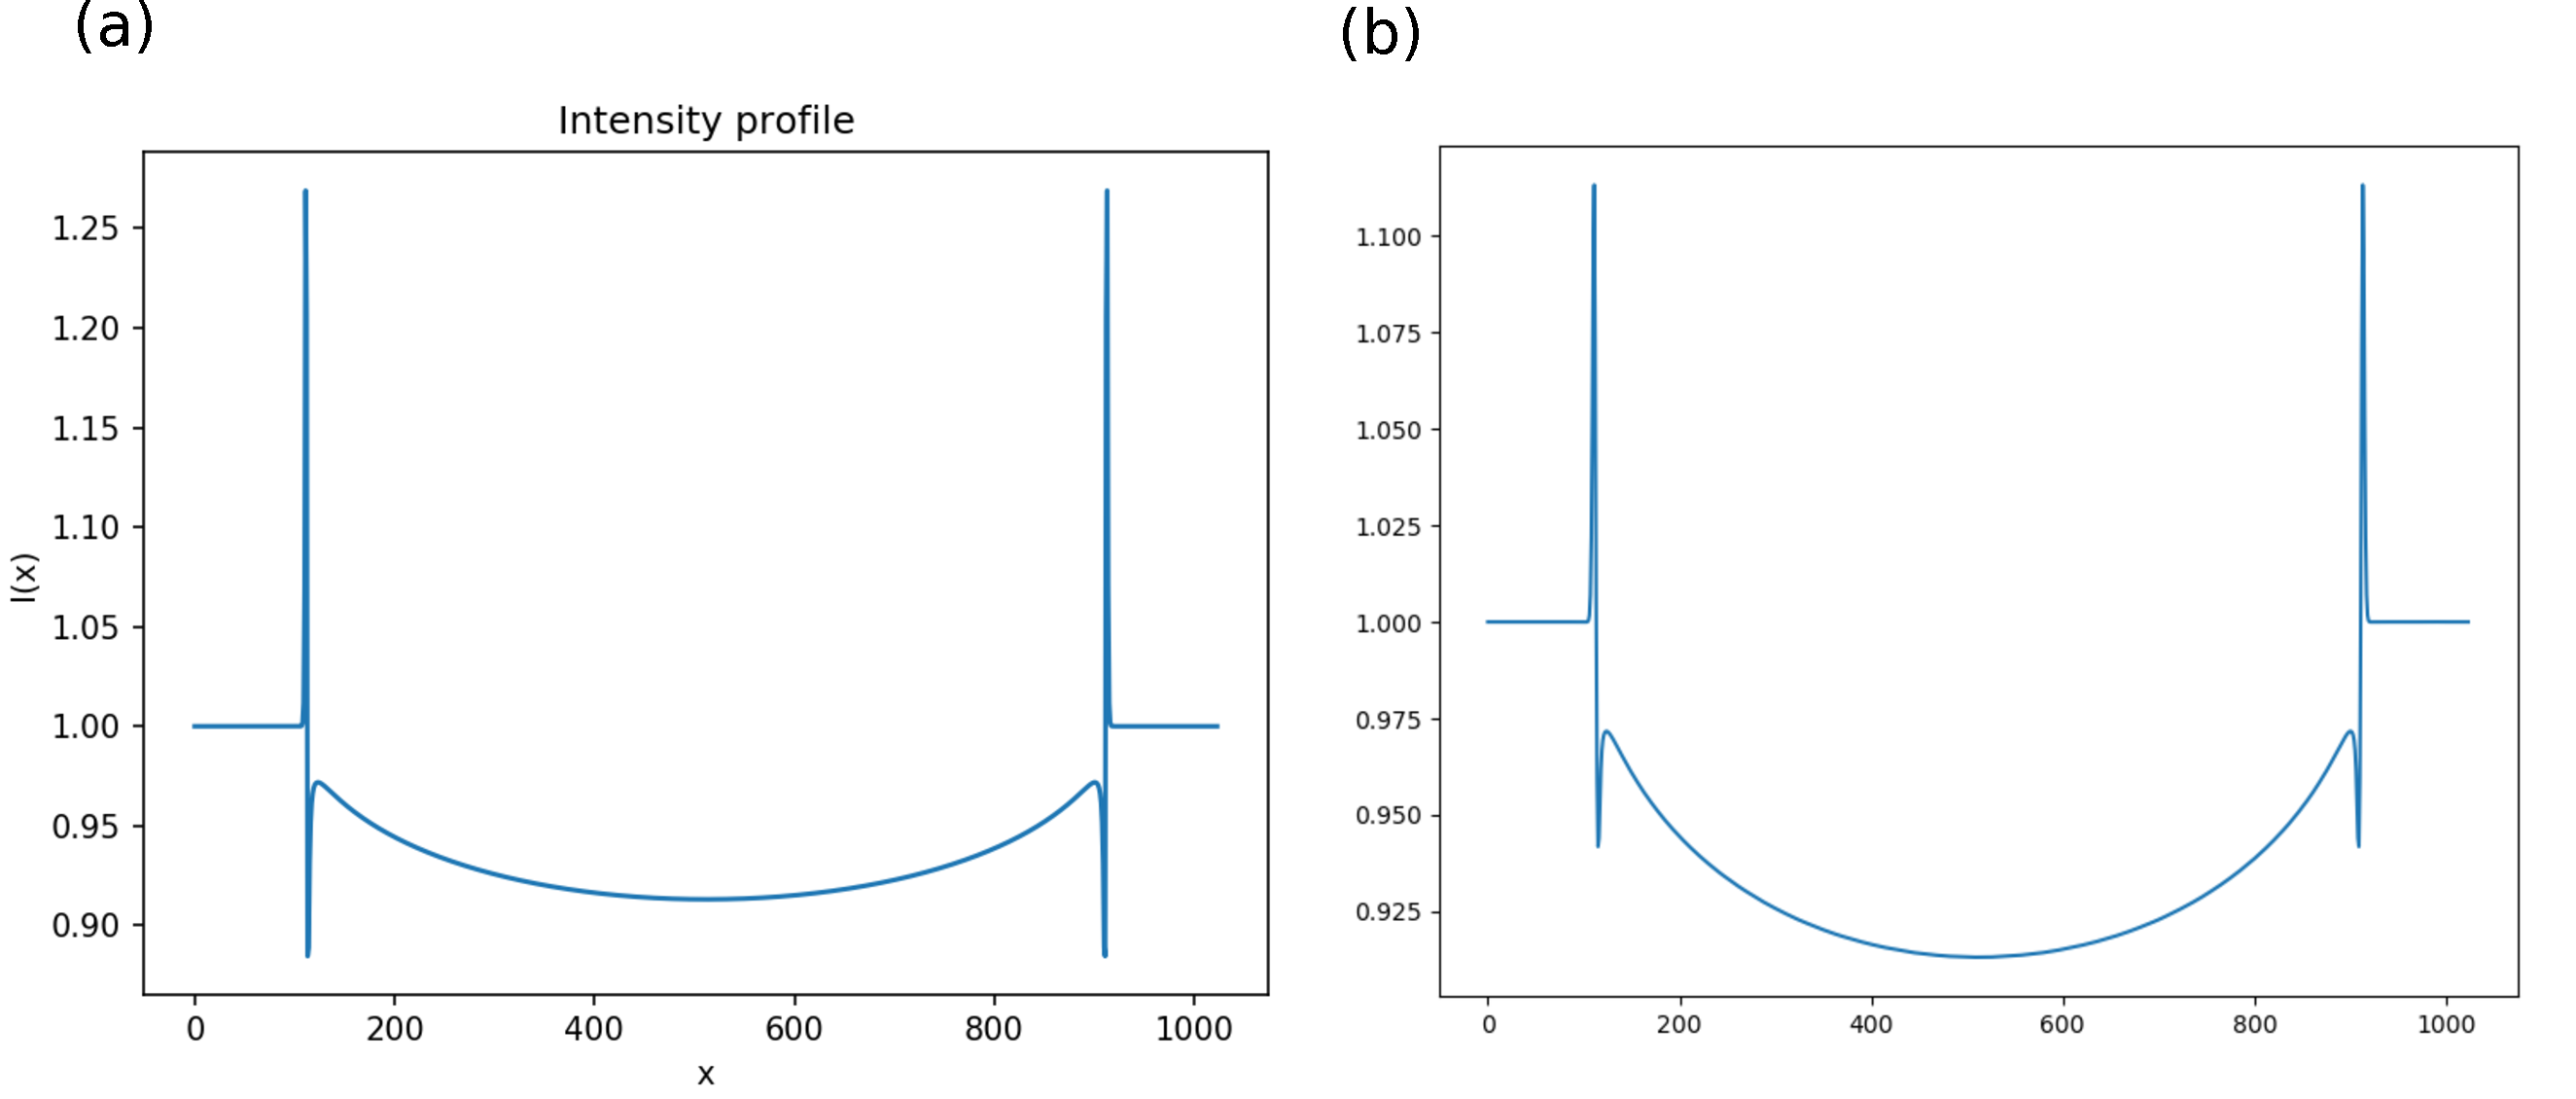
\includegraphics[width=\linewidth]{RK_TEST.pdf}
\captionof{figure}{Phase contrast cross sections obtained by testing: (a) my finite differences with Runge-Kutta propagation method and (b) the TIE propagation method developed by the X-ray imaging group. The input parameters and spatial discretisation codes were identical in both (a) and (b). The parameters were for a single cylinder with a radius of  $R = 2$ mm. The X-ray energy used was $50$keV. The refractive index decrement for the water cylinder is $\delta = 9.21425\times 10^{-8}$ and an attenuation coefficient of $\mu = 22.69615\mathrm{m^{-1}}$. In figure (a), the sigmoid function blurred $0.14$ pixels over the edge of the imaged cylinder.  
The spatial discretisation arrays used in (a) and (b) were both 2D arrays: $x, y = 1024, 1024$ and, the pixel size was$5\mathrm{\mu}$ m.The propagation distance used was $z = 1$ m.}
\end{Figure}
\begin{Figure}\label{fig:3.5}
\centering
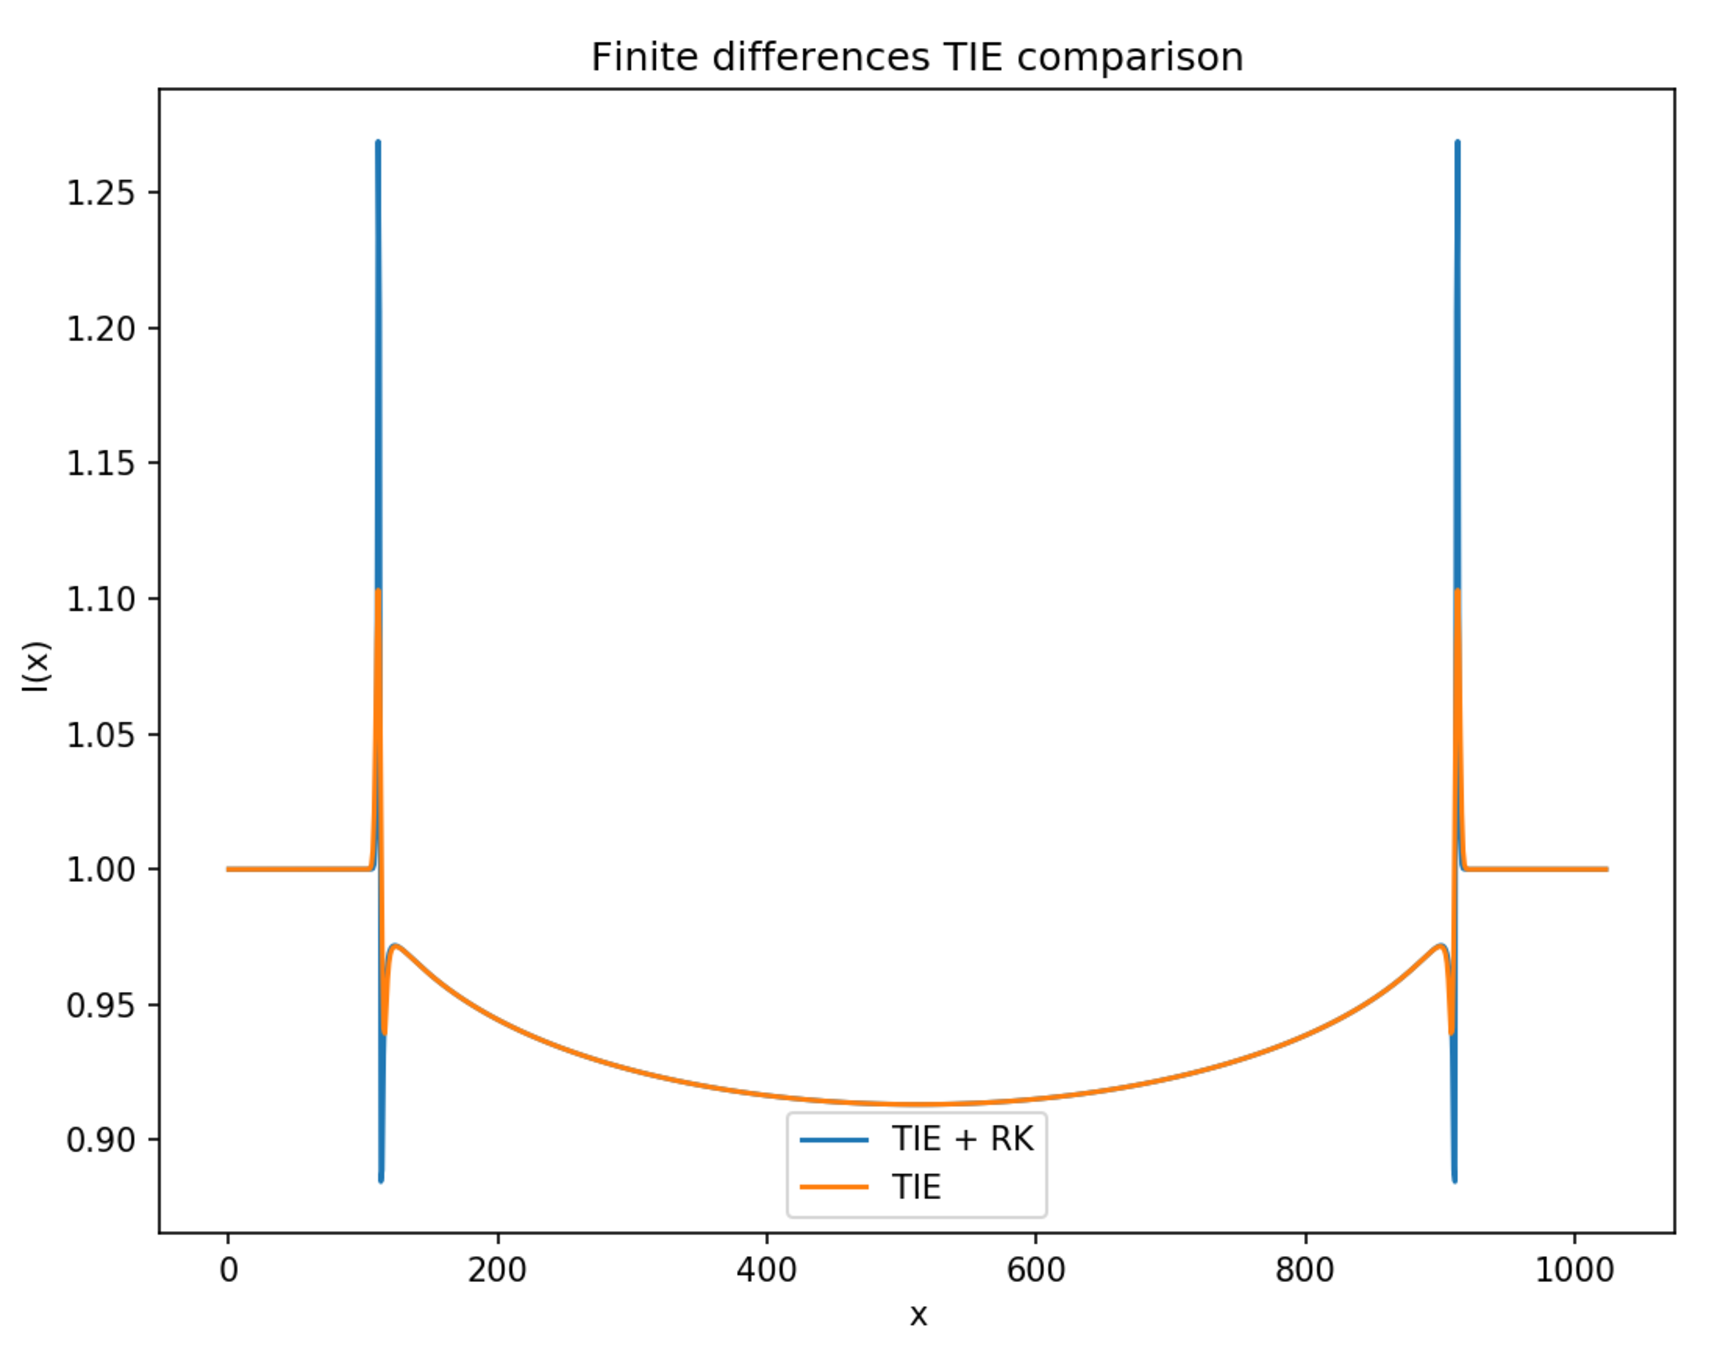
\includegraphics[width=0.6\linewidth]{RK_TEST_difference.pdf}
\captionof{figure}{Phase contrast cross sections as per figure \ref{fig:3} plotted together to quantify the difference in phase contrast results. The difference in the brightness peaks and troughs between these results are $I_{\mathrm{peak}} = 0.165$ and $I_{\mathrm{trough}} = -0.055$ respectively.}
\end{Figure}
Further tests need to be done to prove definitely that the addition of the Runge-Kutta algorithm for spatial propagation can drastically improve phase contrast. Nevertheless, the result shown in figures \ref{fig:3} and \ref{fig:3.5} is interesting because it is possible that my method could even improve phase retrieval results.

\subsection{Density difference test: water and ice}
To test if there is a density dependence in phase contrast, I first used a sample consisting of two cylinders with the outermost one made of water and the innermost one made of ice.
\begin{Figure}\label{fig:4}
\centering
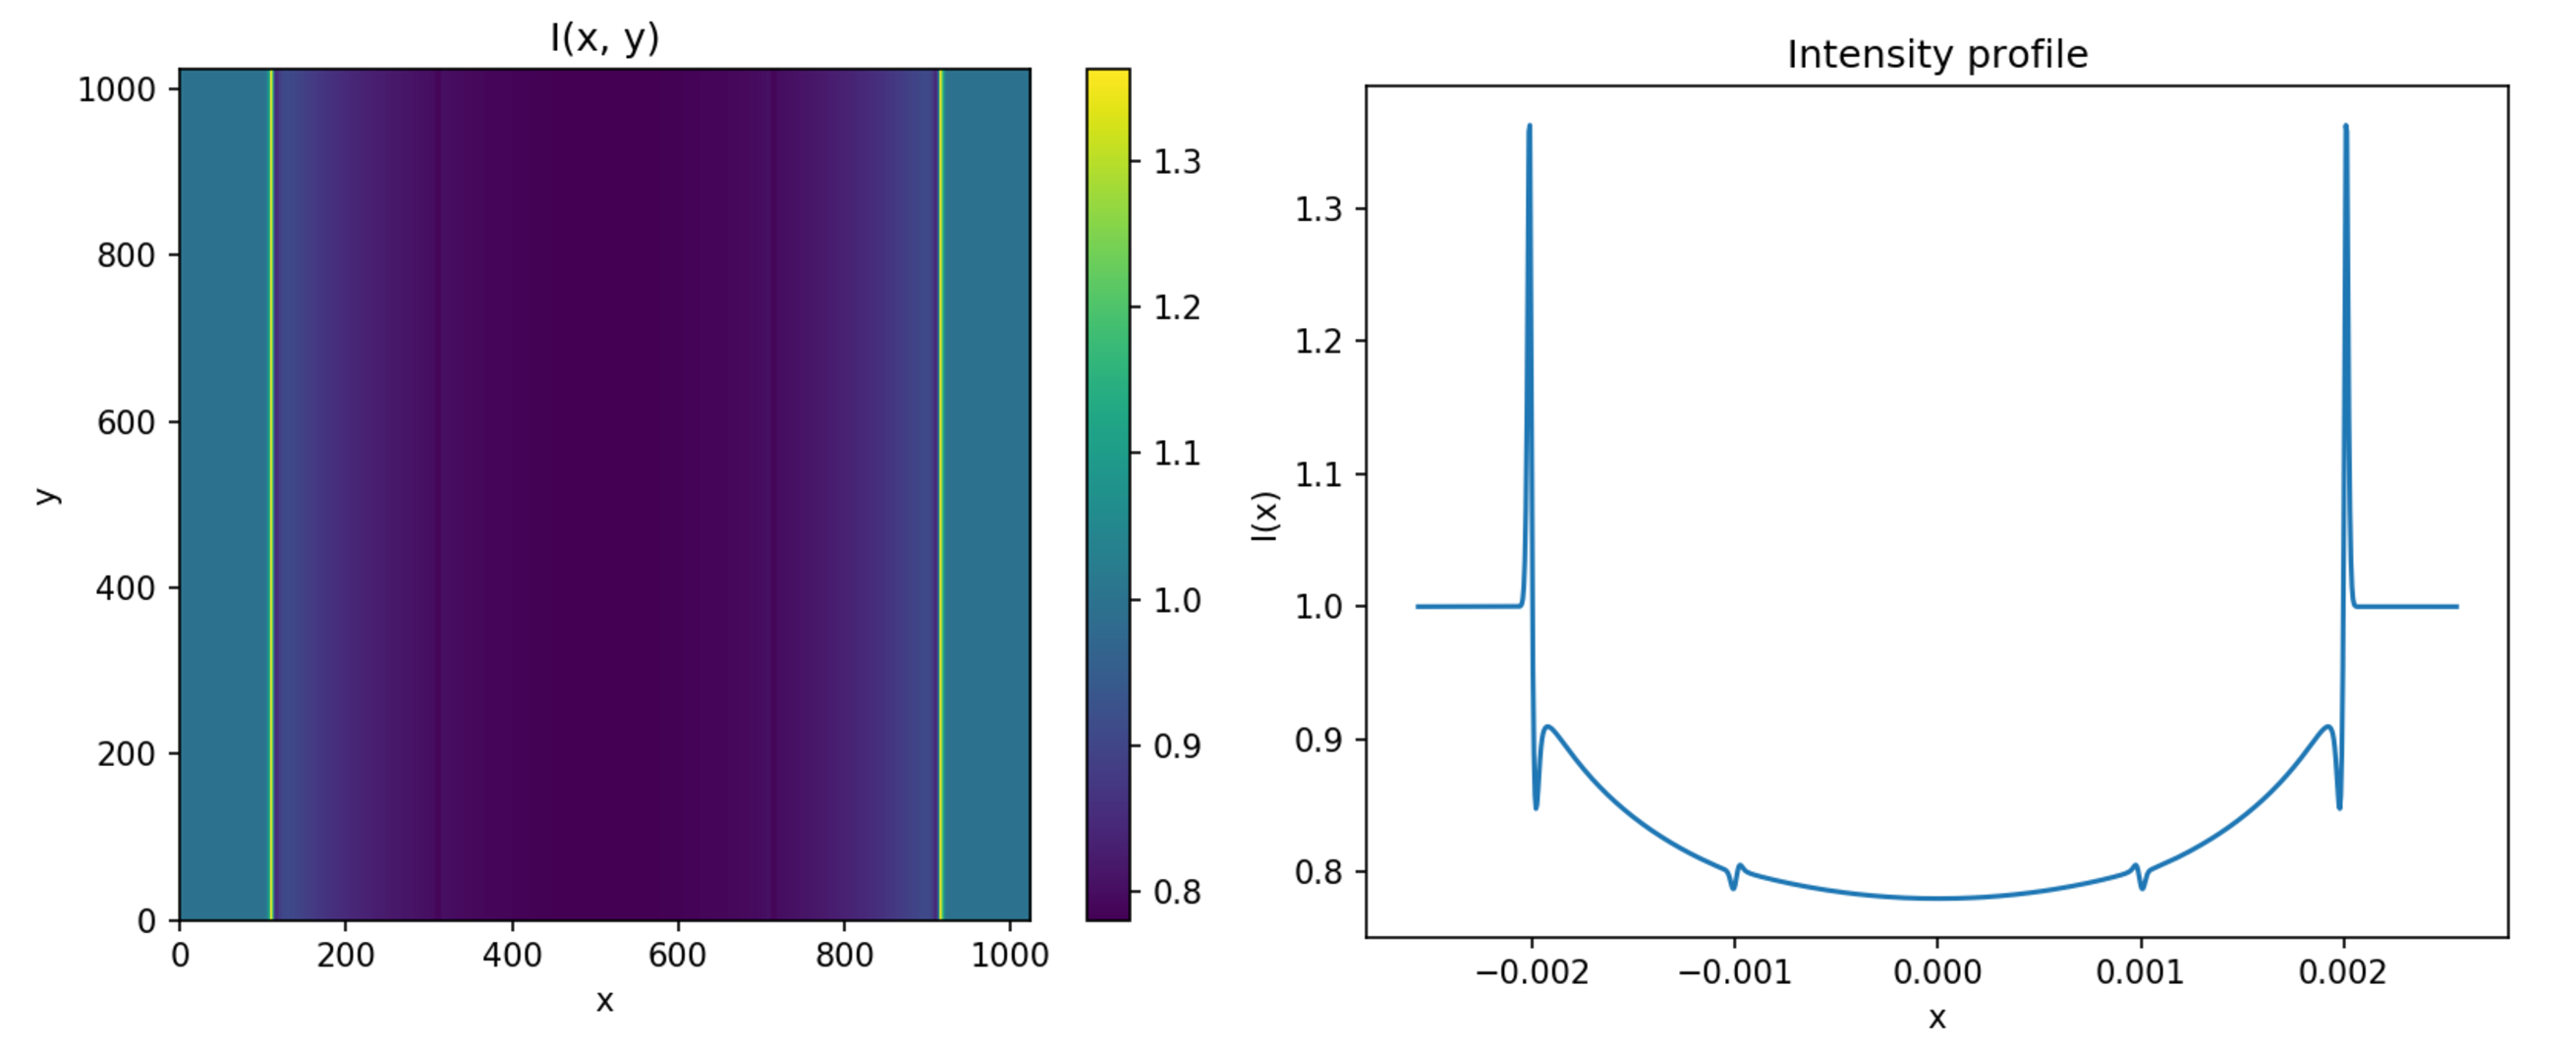
\includegraphics[width=\linewidth]{ice_water_AS.pdf}
\captionof{figure}{Phase contrast image and cross section obtained with the angular spectrum formulation method developed by the X-ray imaging group. The X-ray energy used in this simulation was $E = 22.1629$ keV. The water cylinder has a refractive index decrement $\delta_w = 4.69337\times10^{-7}$, the attenuation coefficient of water is $\mu_w = 64.55083~\mathrm{m^{-1}}$. The ice cylinder has a refractive index decrement $\delta_i = 4.31790\times10^{-7}$, and attenuation coefficient $\mu_i = 59.38677~\mathrm{m^{-1}}$. The density difference between these materials is $\Delta \rho = 0.08~\mathrm{g cm^{-3}}$. The cylinder's radii were $R_w = 2$mm and $R_i = 1$mm. The propagation distance used was $z = 2.5$ m.}
\end{Figure}
With the result in figure \ref{fig:4}. I demonstrate that any changes in material density throughout the imaged sample do affect the imaging process, and therefore the stability the propagation based imaging algorithm developed by Paganin et al. (2002) is actually dependent on the ratio of the differences in the refraction and attenuation coefficients $\Delta \delta$ and $\Delta \mu$ of the imaged materials.
In another simulation I made, I take into account the apparatus parameters and the resolution of the detector used in the lab. I made this simulation to see whether or not we would be able to see the any small fringes in a real experiment. Using magnification factors we would use in the lab (i.e. $2.5$X and $4.0$X) and our photon detector dimensions I resized the spatial array boundaries to match those of the detector. I also scaled the pixel size to match the pixels in the photon detector. I did this so that the pixels in the object plane are adequately sized given the expected size of the pixels in the detector plane. I also calculated the effective propagation distance by dividing the simulation propagation distance by the desired magnification factor.
\begin{Figure}\label{fig:5}
\centering
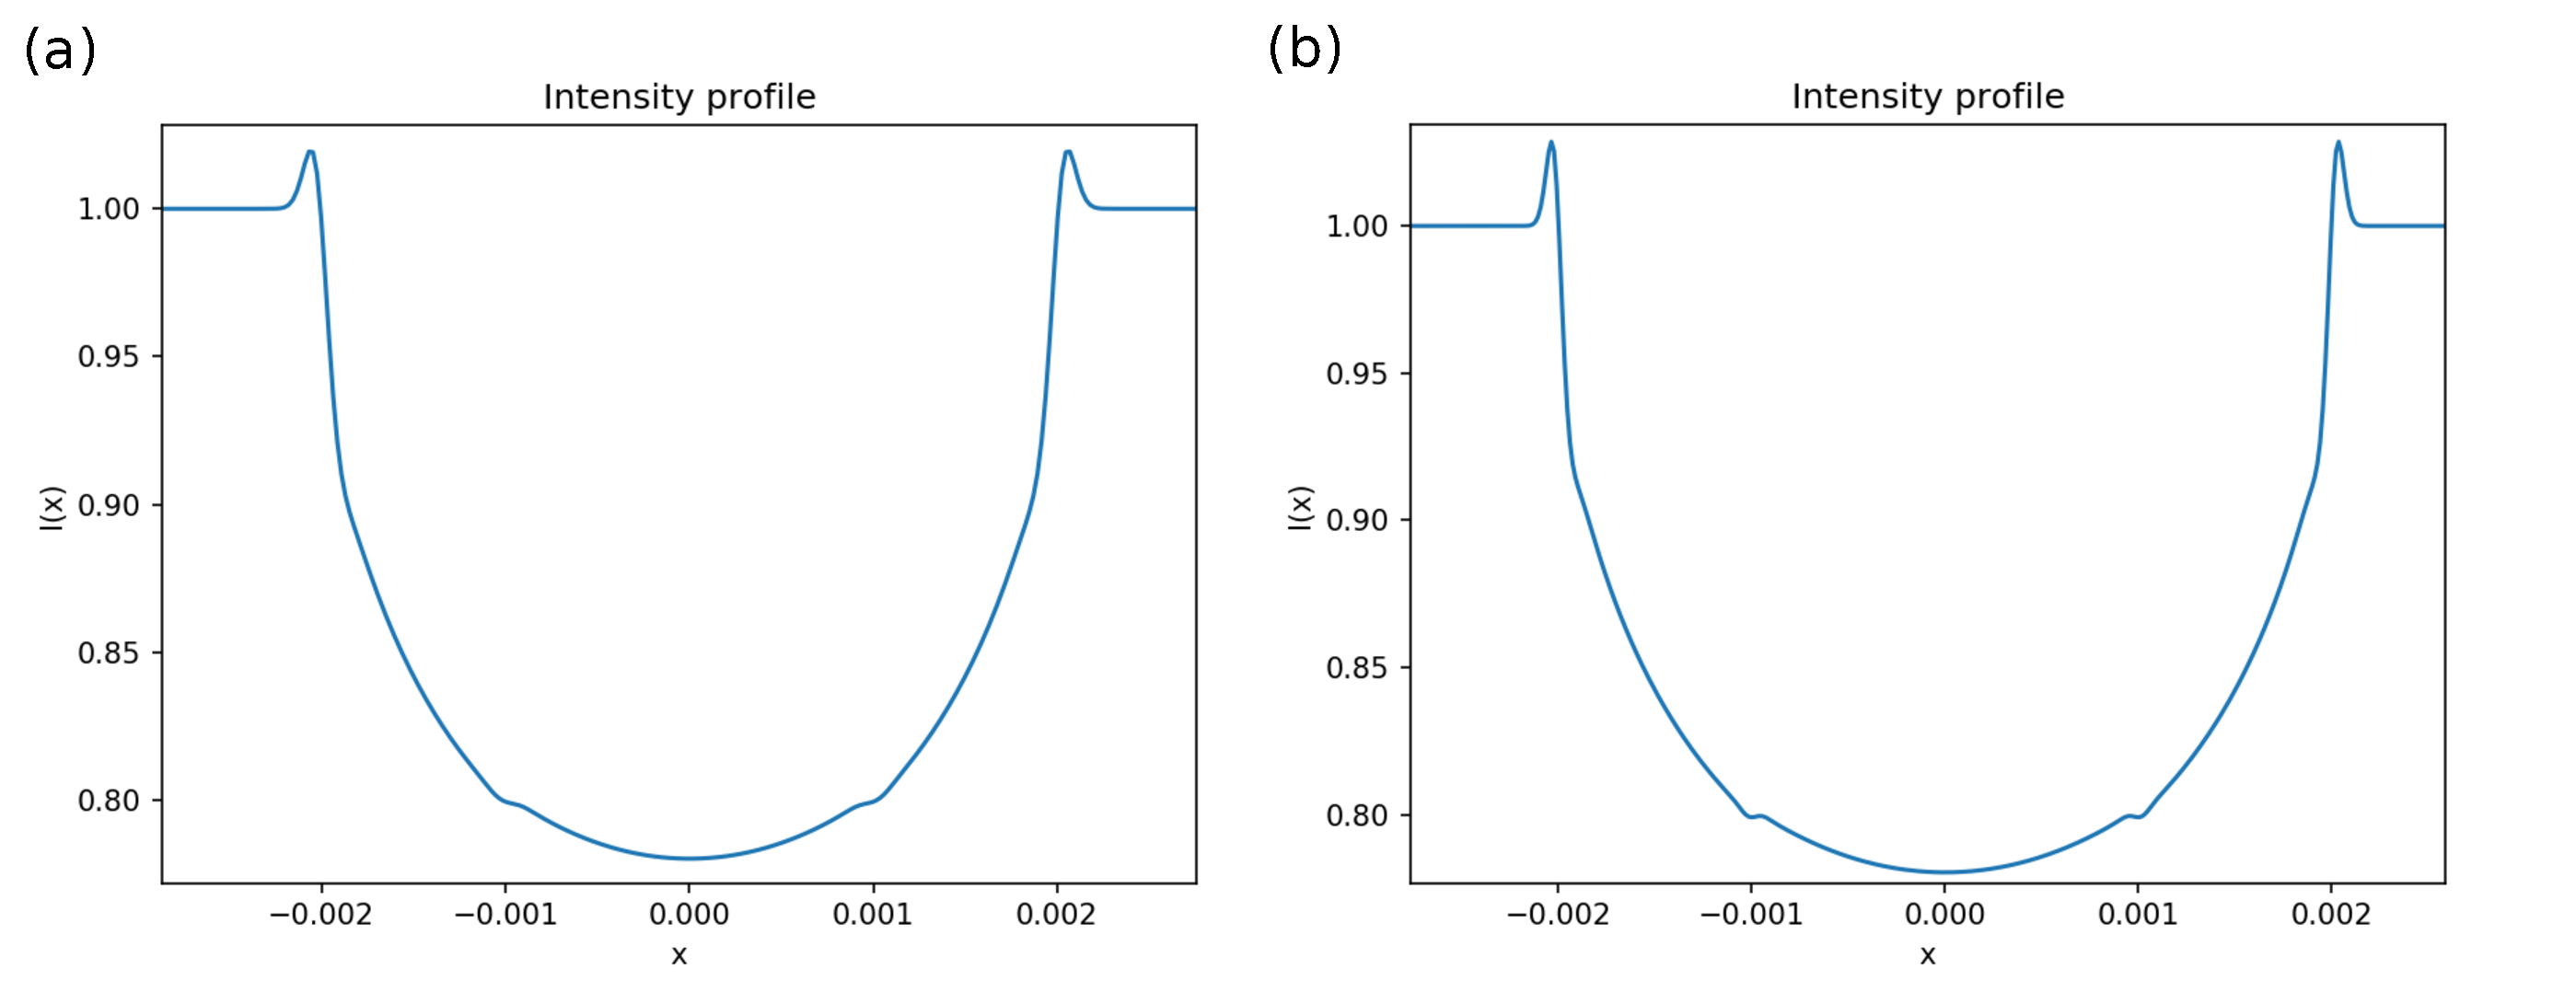
\includegraphics[width=\linewidth]{LAB_ice_water_AS_2_magnifications.pdf}
\captionof{figure}{Phase contrast cross sections were obtained with parameters equal to those in the simulation in figure \ref{fig:4}.}
\end{Figure}
The plan was to test these results experimentally, but given that the phase contrast fringes observable in figure \ref{fig:5} were so small, we decided against doing the experiment, since we would not observe much in a lab setting. 
\subsection{Density difference test: Grey matter and white matter}
To continue my tests of the importance of density in phase contrast, I assume in figure \ref{fig:6}. that grey and white matter have the same chemical compositions but distinct densities.
\begin{Figure}\label{fig:6}
\centering
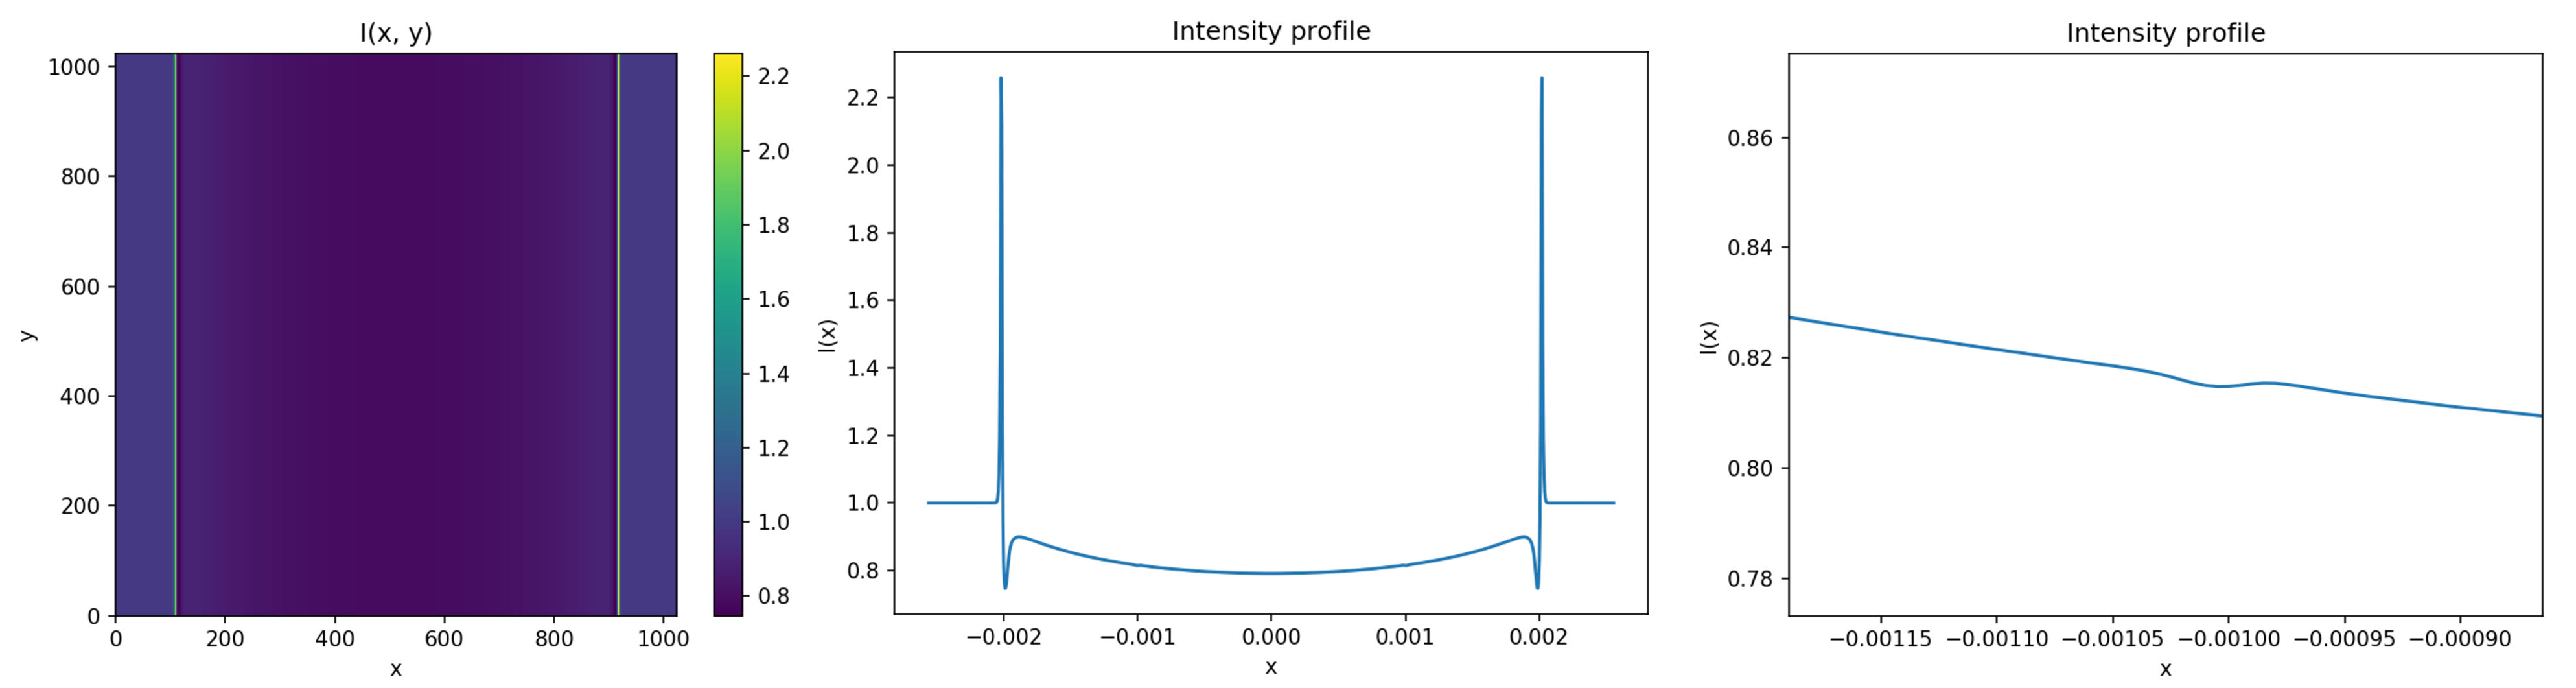
\includegraphics[width=\linewidth]{pessimistic_case.pdf}
\captionof{figure}{Phase contrast image (a), cross section (b), and enhanced view of one the inner cylinder phase contrast fringes (c) obtained with the angular spectrum formulation method as developed by the X-ray imaging group. In (c) it can be seen that the phase contrast fringes from the inner cylinder are extremely small but can still be observed when the image in (b) is amplified enough. The X-ray energy is $E = 24$ keV. The grey matter cylinder has a refractive index decrement $\delta_{GM} = 4.1345\times10^{-7}$, and the attenuation coefficient of grey matter is $\mu_{GM} = 58.2978~\mathrm{m^{-1}}$. The white matter cylinder has a refractive index decrement $\delta_{WM} = 411.87\times10^{-7}$ and its attenuation coefficient $\mu_{WM}= 58.0747~\mathrm{m^{-1}}$. The density difference between these materials is $\Delta \rho = 0.004~\mathrm{g cm^{-3}}$\cite{ITIS}. The cylinders' radii were $R_{GM} = 2$ mm and $R_{WM} = 1$ mm. The propagation distance used was $z = 2.5$ m.}
\end{Figure}
My simulations demonstrate that even a small density difference like the one seen in \ref{fig:6} can produce phase contrast fringes. Nevertheless, my simulations only consider perfect data, therefore the fringes would be too small to see using real sample materials in a lab experiment.

\subsection{Chemical difference test: Grey matter and white matter}
\begin{Figure}\label{fig:7}
\centering
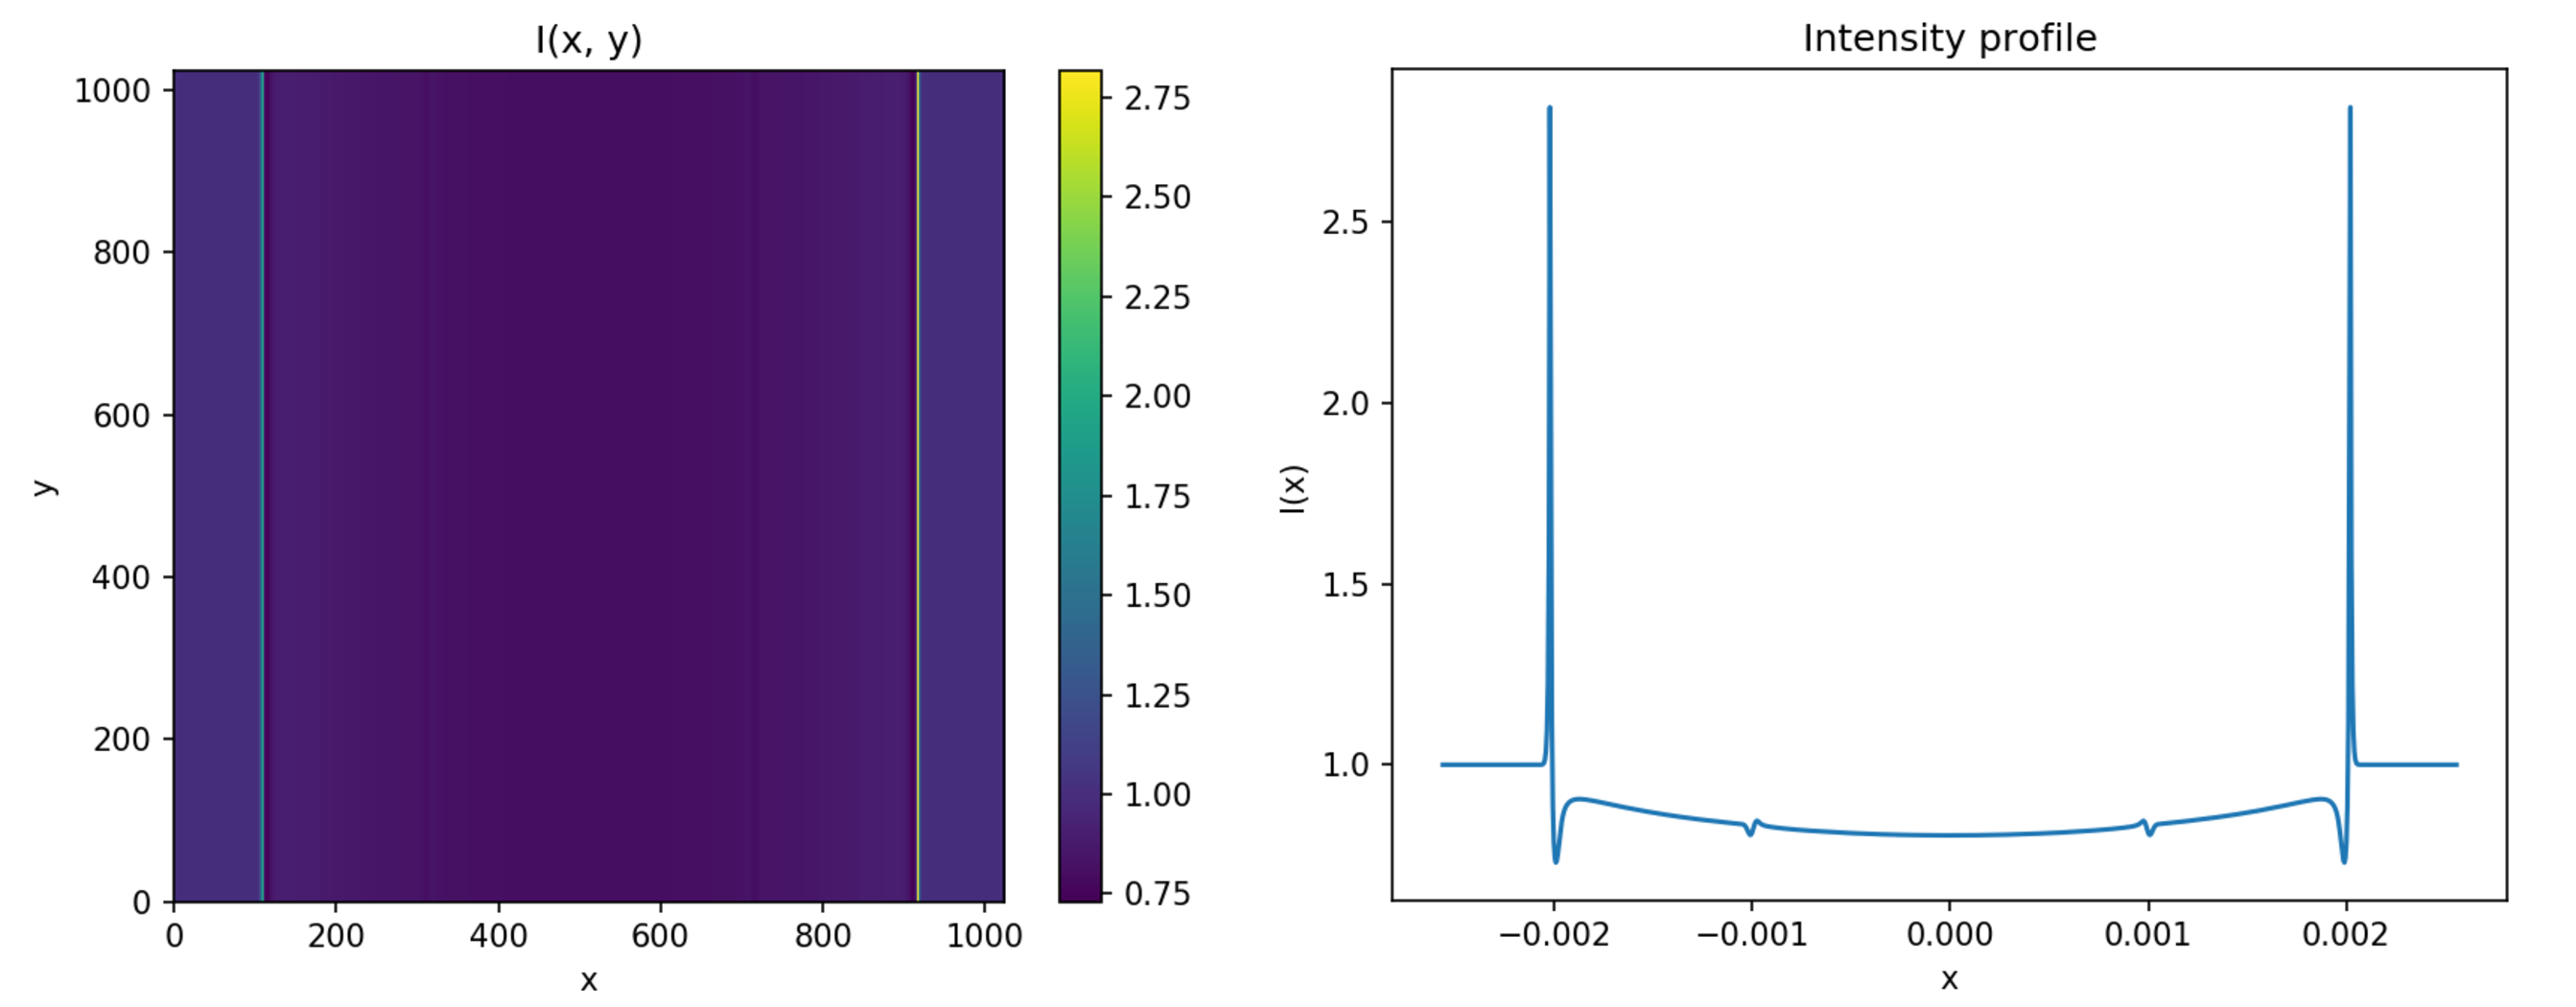
\includegraphics[width=\linewidth]{optimistic_case.pdf}
\captionof{figure}{Phase contrast image and phase contrast cross section obtained with the angular spectrum formulation method developed by the X-ray imaging group. The X-ray energy used in this simulation was $E = 24$keV. The grey matter cylinder has a refractive index decrement $\delta_{GM} = 4.591\times10^{-7}$, the attenuation coefficient of grey matter is $\mu_{GM} = 52\mathrm{m^{-1}}$\cite{Linda}. The white matter cylinder has a refractive index decrement $\delta_{WM} = 4.2631\times10^{-7}$ and attenuation coefficient $\mu_{WM}= 56~\mathrm{m^{-1}}$\cite{Linda}. The cylinders' radii were $R_{GM} = 2$ mm and $R_{WM} = 1$ mm. The propagation distance used was $z = 2.5$m.}
\end{Figure}

\section{Future Plans}

To definitely demonstrate that adding the Runge-Kutta algorithm for spatial propagation drastically improves phase contrast as per figure \ref{fig:3}, I must test my method against other propagation methods used by the X-ray group. These methods include the angular spectrum formulation and Fresnel propagation. If my method consistently yields higher phase contrast, I need to investigate whether higher phase contrast is an accurate measure that would increase the chances of improving phase retrieval results.

I aim to finish my density simulations by creating a graphic user interface (GUI) that allows the user to modify interactively the density parameters of the imaged concentric cylinders in the simulation. The goal is to make an easily operated visual representation of the changes in phase and intensity of the X-rays as they interact with the imaged object in-situ.

My supervisor and I are planning to test an X-ray target made of silver which has been obtained for the laboratory apparatus. I need to make simulations using the characteristic radiation spectrum of silver and see how the phase contrast fringes behave when isolating monochromatic X-ray fringes and comparing them to each other. My aim is to eventually obtain real laboratory data and analyse it to compare the efficacy of the new silver target to that of the classic tungsten target currently used in the apparatus.

\section{Conclusion}
The aim of my project is to investigate how the phase of incident X-rays changes as the density of distinct sample materials in an arbitrary imaging system changes. I demonstrate that any changes in material density throughout the imaged sample affect the imaging process. The eventual goals of these simulations is to verify if successful phase retrieval can be done of the imaged objects given their variable densities. This report presents a brief outline of the theory behind coherent X-ray imaging, a description of my current progress, and a brief description of my future aims.

\bibliography{mybib}
\bibliographystyle{unsrt}
\end{document}
